\documentclass[journal,12pt,twocolumn]{IEEEtran}
\usepackage{setspace}
\usepackage{gensymb}
\usepackage{xcolor}
\usepackage{caption}
%\usepackage{subcaption}
%\doublespacing
\singlespacing
%\usepackage{graphicx}
%\usepackage{amssymb}
%\usepackage{relsize}
\usepackage[cmex10]{amsmath}
\usepackage{mathtools}
%\usepackage{amsthm}
%\interdisplaylinepenalty=2500
%\savesymbol{iint}
%\usepackage{txfonts}
%\restoresymbol{TXF}{iint}
%\usepackage{wasysym}
\usepackage{hyperref}
\usepackage{amsthm}
\usepackage{mathrsfs}
\usepackage{txfonts}
\usepackage{stfloats}
\usepackage{cite}
\usepackage{cases}
\usepackage{subfig}
%\usepackage{xtab}
\usepackage{longtable}
\usepackage{multirow}
%\usepackage{algorithm}
%\usepackage{algpseudocode}
%\usepackage{enumerate}
\usepackage{enumitem}
\usepackage{mathtools}
%\usepackage{iithtlc}
%\usepackage[framemethod=tikz]{mdframed}
\usepackage{listings}
\usepackage{polynom}

%\usepackage{wasysym}
%\newcounter{MYtempeqncnt}
\DeclareMathOperator*{\Res}{Res}
%\renewcommand{\baselinestretch}{2}
\renewcommand\thesection{\arabic{section}}
\renewcommand\thesubsection{\thesection.\arabic{subsection}}
\renewcommand\thesubsubsection{\thesubsection.\arabic{subsubsection}}

\renewcommand\thesectiondis{\arabic{section}}
\renewcommand\thesubsectiondis{\thesectiondis.\arabic{subsection}}
\renewcommand\thesubsubsectiondis{\thesubsectiondis.\arabic{subsubsection}}

%\renewcommand{\labelenumi}{\textbf{\theenumi}}
%\renewcommand{\theenumi}{P.\arabic{enumi}}

% correct bad hyphenation here
\hyphenation{op-tical net-works semi-conduc-tor}

\makeatletter
\def\pld@CF@loop#1+{%
	\ifx\relax#1\else
	\begingroup
	\pld@AccuSetX11%
	\def\pld@frac{{}{}}\let\pld@symbols\@empty\let\pld@vars\@empty
	\pld@false
	#1%
	\let\pld@temp\@empty
	\pld@AccuIfOne{}{\pld@AccuGet\pld@temp
		\edef\pld@temp{\noexpand\pld@R\pld@temp}}%
	\pld@if \pld@Extend\pld@temp{\expandafter\pld@F\pld@frac}\fi
	\expandafter\pld@CF@loop@\pld@symbols\relax\@empty
	\expandafter\pld@CF@loop@\pld@vars\relax\@empty
	\ifx\@empty\pld@temp
	\def\pld@temp{\pld@R11}%
	\fi
	\global\let\@gtempa\pld@temp
	\endgroup
	\ifx\@empty\@gtempa\else
	\pld@ExtendPoly\pld@tempoly\@gtempa
	\fi
	\expandafter\pld@CF@loop
	\fi}
\def\pld@CMAddToTempoly{%
	\pld@AccuGet\pld@temp\edef\pld@temp{\noexpand\pld@R\pld@temp}%
	\pld@CondenseMonomials\pld@false\pld@symbols
	\ifx\pld@symbols\@empty \else
	\pld@ExtendPoly\pld@temp\pld@symbols
	\fi
	\ifx\pld@temp\@empty \else
	\pld@if
	\expandafter\pld@IfSum\expandafter{\pld@temp}%
	{\expandafter\def\expandafter\pld@temp\expandafter
		{\expandafter\pld@F\expandafter{\pld@temp}{}}}%
	{}%
	\fi
	\pld@ExtendPoly\pld@tempoly\pld@temp
	\pld@Extend\pld@tempoly{\pld@monom}%
	\fi}
\makeatother

\lstset{
	language=Python,
	frame=single, 
	breaklines=true,
	columns=fullflexible
}

\begin{document}
	
	\theoremstyle{definition}
	\newtheorem{theorem}{Theorem}[section]
	\newtheorem{problem}{Problem}
	\newtheorem{proposition}{Proposition}[section]
	\newtheorem{lemma}{Lemma}[section]
	\newtheorem{corollary}[theorem]{Corollary}
	\newtheorem{example}{Example}[section]
	\newtheorem{definition}{Definition}[section]
	%\newtheorem{algorithm}{Algorithm}[section]
	%\newtheorem{cor}{Corollary}
	\newcommand{\BEQA}{\begin{eqnarray}}
	\newcommand{\EEQA}{\end{eqnarray}}
	\newcommand{\define}{\stackrel{\triangle}{=}}
	\bibliographystyle{IEEEtran}
	%\bibliographystyle{ieeetr}
	\providecommand{\nCr}[2]{\,^{#1}C_{#2}} % nCr
	\providecommand{\nPr}[2]{\,^{#1}P_{#2}} % nPr
	\providecommand{\mbf}{\mathbf}
	\providecommand{\pr}[1]{\ensuremath{\Pr\left(#1\right)}}
	\providecommand{\qfunc}[1]{\ensuremath{Q\left(#1\right)}}
	\providecommand{\sbrak}[1]{\ensuremath{{}\left[#1\right]}}
	\providecommand{\lsbrak}[1]{\ensuremath{{}\left[#1\right.}}
	\providecommand{\rsbrak}[1]{\ensuremath{{}\left.#1\right]}}
	\providecommand{\brak}[1]{\ensuremath{\left(#1\right)}}
	\providecommand{\lbrak}[1]{\ensuremath{\left(#1\right.}}
	\providecommand{\rbrak}[1]{\ensuremath{\left.#1\right)}}
	\providecommand{\cbrak}[1]{\ensuremath{\left\{#1\right\}}}
	\providecommand{\lcbrak}[1]{\ensuremath{\left\{#1\right.}}
	\providecommand{\rcbrak}[1]{\ensuremath{\left.#1\right\}}}
	\theoremstyle{remark}
	\newtheorem{rem}{Remark}
	\newcommand{\sgn}{\mathop{\mathrm{sgn}}}
	\providecommand{\abs}[1]{\left\vert#1\right\vert}
	\providecommand{\res}[1]{\Res\displaylimits_{#1}} 
	\providecommand{\norm}[1]{\lVert#1\rVert}
	\providecommand{\mtx}[1]{\mathbf{#1}}
	\providecommand{\mean}[1]{E\left[ #1 \right]}
	\providecommand{\fourier}{\overset{\mathcal{F}}{ \rightleftharpoons}}
	\providecommand{\ztrans}{\overset{\mathcal{Z}}{ \rightleftharpoons}}
	%\providecommand{\hilbert}{\overset{\mathcal{H}}{ \rightleftharpoons}}
	\providecommand{\system}{\overset{\mathcal{H}}{ \longleftrightarrow}}
	%\newcommand{\solution}[2]{\textbf{Solution:}{#1}}
	\newcommand{\solution}{\noindent \textbf{Solution: }}
	\providecommand{\dec}[2]{\ensuremath{\overset{#1}{\underset{#2}{\gtrless}}}}
	%\numberwithin{equation}{section}
	%\numberwithin{equation}{subsection}
	%\numberwithin{problem}{subsection}
	%\numberwithin{definition}{subsection}
	%\renewcommand{\thefigure}{\theproblem.\arabic{figure}}
	%\renewcommand{\thefigure}{\theproblem}
	\renewcommand{\thefigure}{\arabic{figure}}
	\makeatletter
	\@addtoreset{figure}{section}
	\makeatother
	%\numberwithin{figure}{subsection}
	\def\putbox#1#2#3{\makebox[0in][l]{\makebox[#1][l]{}\raisebox{\baselineskip}[0in][0in]{\raisebox{#2}[0in][0in]{#3}}}}
	\def\rightbox#1{\makebox[0in][r]{#1}}
	\def\centbox#1{\makebox[0in]{#1}}
	\def\topbox#1{\raisebox{-\baselineskip}[0in][0in]{#1}}
	\def\midbox#1{\raisebox{-0.5\baselineskip}[0in][0in]{#1}}
	\vspace{3cm}
	\title{Assignment - 2}
	\author{Vaibhav Ramola} 
	% make the title area
	\maketitle
	%\newpage
	%\renewcommand{\thefigure}{\thesection.\theenumi}
	%\renewcommand{\thetable}{\thesection.\theenumi}
	%\renewcommand{\thefigure}{\theenumi}
	%\renewcommand{\thetable}{\theenumi}
	%\renewcommand{\theequation}{\thesection}
	\bigskip
	\begin{abstract}
		This document contains the solution to Exercise 3.31 (a) of Oppenheim.
	\end{abstract}
	
	\problem  Determine the z-transform and region of convergnce, and sketch the pole-zero diagram for the following sequence : 
	\begin{equation*}
	x[n] = a^{n}u[n] + b^{n}u[n] + c^{n}u[-n-1], \quad |a| < |b| < |c|
	\end{equation*}
	\solution
	\begin{align*}
	&x[n] =  a^{n}u[n] + b^{n}u[n] + c^{n}u[-n-1] \quad |a|<|b|<|c|\\
	&X(z) =  \frac{1}{1-az^{-1}} + \frac{1}{1-bz^{-1}} - \frac{1}{1-cz^{-1}} \quad |b|<|z|<|c|\\
	&X(z) =  \frac{1 - 2cz^{-1} + (bc + ac - ab)z^{-2}}{(1 - az^{-1})(1 - bz^{-1})(1 - cz^{-1})}
	\quad |b|<|z|<|c|\\
	&\text{Poles : a,b,c}\\
	&\text{Zeros : $z_{1}$, $z_{2}$, $\infty$ where $z_{1}$ and $z_{2}$ are roots of numerator quadratic}\\
	\end{align*}
	\begin{figure}[!ht]
		\centering
		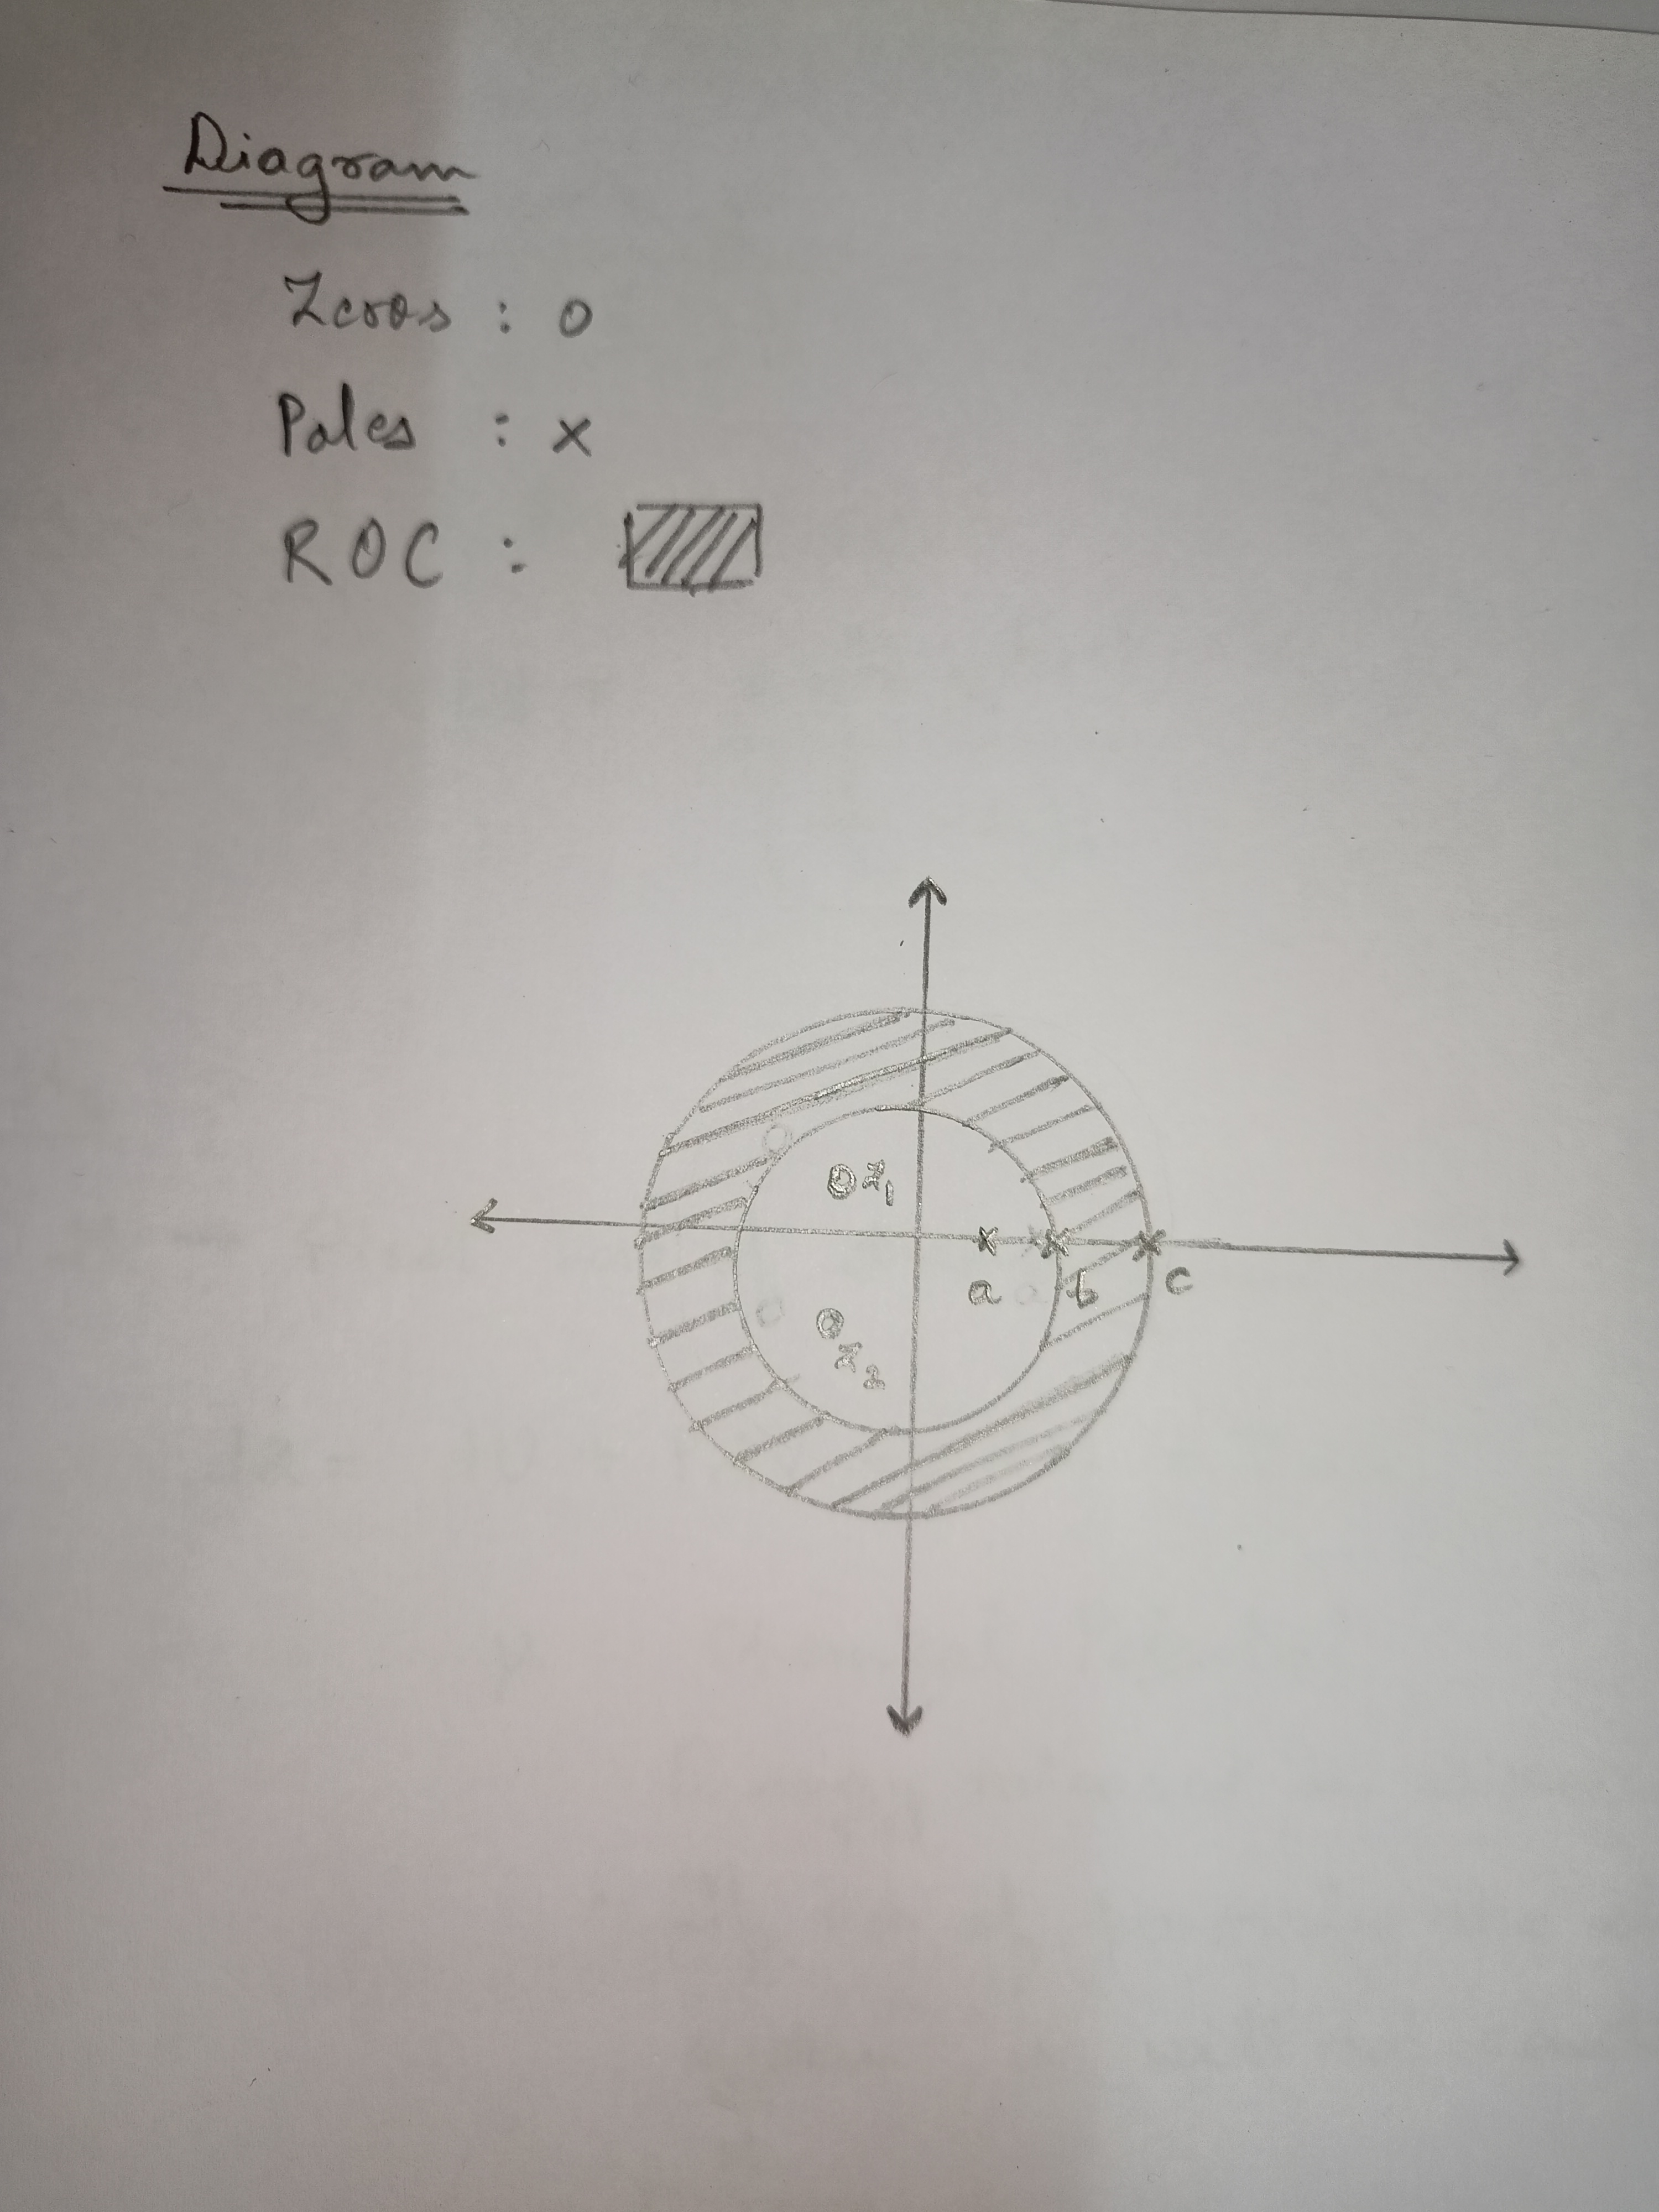
\includegraphics[width=225 pt]{diagram.jpg}
		\label{fig:ques}
	\end{figure} 
\end{document}